\documentclass[UTF8, a4paper]{ctexart}
\usepackage[margin=1in]{geometry} % 页边距调整
\usepackage{ctex}
\usepackage{array, amsmath, amssymb}

% subsection subsection_name (end)

\usepackage{booktabs, tabularx, multirow, multicol} % 表格拓展支持
\usepackage{graphicx, subfigure, float} % 图片排版支持

\usepackage{algorithm, algpseudocode} % 伪代码支持
\renewcommand{\algorithmicrequire}{\textbf{Input:}}  
\renewcommand{\algorithmicensure}{\textbf{Output:}} 

\usepackage{tikz, mathpazo} % 基本绘图支持
\usepackage{flowchart} % 流程图支持
\usepackage{pgf-umlcd} % UML类图支持
\usetikzlibrary{arrows, shapes, chains, shapes.geometric}

\usepackage{listings} % 代码块支持
\usepackage{xcolor}
\lstset{
	language		= c++,
	backgroundcolor	= \color{white},
	basicstyle		= \footnotesize\ttfamily,
	keywordstyle	= \color{blue},
	stringstyle		= \color{red!58!blue!82}\ttfamily,
	commentstyle	= \color{darkgray},
	rulesepcolor	= \color{red!20!green!20!blue!20},
	columns			= fullflexible,
	breaklines		= true,
	captionpos		= b,
	tabsize			= 4,
	frame			= single,
	escapeinside	= {\%*}{*)}
}
%%示例
% \begin{lstlisting}[caption={}]
% #include <iostream>
% int main(int argc, char *argv[]) {
% 	std::cout << "Hello World!" << std::endl;
% 	return 0;
% }
% \end{lstlisting}

\usepackage{datetime} %日期
\renewcommand{\today}{\number\year{年}\number\month{月}\number\day{日}}

\begin{document}

\begin{center}
	\zihao{3}《数据结构》实验报告
\end{center}
\zihao{5}

\newcolumntype{Y}{>{\raggedleft\arraybackslash}X}
\noindent\begin{tabularx}{\textwidth}{XcY}
	  {班 级:}\;\underline{DL062123}
	& {姓 名:}\;\underline{项乔栋}
	& {学 号:}\;\underline{2021302468} \\
	  {邮 箱:}\;\underline{13282135976@sina.cn}
	& {日 期:}\;\underline{\today}
	& {编 号:}\;\underline{DS01}
\end{tabularx}
~\\

\noindent\textbf{$\circledcirc$
实验题目:\quad{合并有序数组}} \par
\noindent\textbf{$\circledcirc$
实验目的:\quad{顺序表的简单使用}} \par
\noindent\textbf{$\circledcirc$
实验内容:\quad{给定元素升序排列的两个数组,合并得到新的升序数组}} \par

\subsection*{一、需求分析}
\noindent\fbox{
\begin{tabularx}{\textwidth}{lY}
\bf{Description}
& \parbox[t]{\linewidth}{
	给定两个按照升序排列的有序数组,请把它们合成一个升序数组并输出。
} \\

\bf{Input}
& \parbox[t]{\linewidth}{
	第一行为第一个有序数组的长度,正整数n ($n\leq{20}$) \\
	第二行为第一个有序数组的n个数字,用空格隔开 \\
	第三行为第二个有序数组的长度,正整数m ($m\leq{20}$) \\
	第四行为第二个有序数组的m个数字,用空格隔开
} \\

\bf{Output}
& \parbox[t]{\linewidth}{
	输出合并后的数组,每个数字占一行
} \\

\bf{Sample Input}
& \fbox{\parbox[t]{\linewidth}{\bf{
	\mbox{3} \\
	\mbox{1 3 7} \\
	\mbox{5} \\
	\mbox{2 4 6 8 10}
}}} \\

\bf{Sample Output}
& \fbox{\parbox[t]{\linewidth}{\bf{
	\mbox{1} \\
	\mbox{2} \\
	\mbox{3} \\
	\mbox{4} \\
	\mbox{6} \\
	\mbox{7} \\
	\mbox{8} \\
	\mbox{10}
}}}
\end{tabularx}}

\subsection*{二、概要设计}
为实现目标功能,使用两个数组a、b分别存储输入数据,并使用新的数组c存储合并结果。 \par
1.\;基本操作: \par
	InputArray() $\rightarrow$ (array,length) \par
	\qquad\textbf{操作结果:}\;存储输入元素的数组与数组长度 \par
	Merge(a, b) $\rightarrow$ array \par
	\qquad\textbf{操作结果:}\;a,b数组的合并结果 \par
	Output(array) $\rightarrow$ void \par
	\qquad\textbf{操作结果:}\;顺序输出数组的元素 \par
2.\;程序模块: \par
1) 主程序 \par
2) IO支持 \par
3) 数组合并 \par
\begin{figure}[H]
	\tikzstyle{module}=[rectangle, draw, thin, fill=white]
	\tikzstyle{terminal}=[module, rounded corners]
	\tikzstyle{testcase}=[draw, diamond, aspect=2, thin]
	\tikzstyle{locate}=[coordinate, on grid]
	\tikzstyle{arrow} = [thick,->,>=stealth]
	\begin{center}\begin{tikzpicture}
		\node(main)[terminal]{主程序};
		\node(main-bottom)[locate, below of=main, node distance=20mm]{};

		\node(io)[module, left of=main-bottom, node distance=16mm]{IO支持};
		\node(io-left)[locate, left of=io, node distance=20mm]{};

		\node(input-right)[locate, above of=io-left, node distance=8mm]{};
		\node(output-right)[locate, below of=io-left, node distance=8mm]{};
		\node(input)[module, left of=input-right, node distance=4mm]{输入模块};
		\node(output)[module, left of=output-right, node distance=4mm]{输出模块};

		\node(input-left)[locate, left of=input, node distance=14mm]{};
		\node(input-to-array-left)[locate, below of=input-left, node distance=28mm]{};

		\node(merge)[module, right of=main-bottom, node distance=16mm]{数组合并};
		\node(merge-bottom)[locate, below of=merge, node distance=12mm]{};

		\node(array-a)[left of=merge-bottom, node distance=12mm]{Array A};
		\node(array-b)[right of=merge-bottom, node distance=12mm]{Array B};
		\node(array-a-below)[locate, below of=array-a, node distance=8mm]{};
		\node(array-b-below)[locate, below of=array-b, node distance=8mm]{};

		\node(merge-right)[locate, right of=merge, node distance=24mm]{};
		\node(array-c-right)[locate, below of=merge-right, node distance=32mm]{};
		\node(array-c)[left of=array-c-right, node distance=24mm]{Array C};
		\node(array-c-left)[locate, left of=array-c, node distance=56mm]{};

		\draw[thick](main.south) -- (main-bottom);
		\draw[arrow](main-bottom) -- (io.east);
		\draw[arrow](main-bottom) -- (merge.west);

		\draw[arrow](io.north) |- (input);
		\draw[arrow](io.south) |- (output);

		\draw[thick](input.west) -- (input-left);
		\draw[thick](input-left) -- (input-to-array-left);
		\draw[thick](input-to-array-left) -- node[anchor=south]{\small{输入数据}} (array-a-below);
		\draw[arrow](array-a-below) -- (array-a);
		\draw[thick](array-a-below) -- (array-b-below);
		\draw[arrow](array-b-below) -- (array-b);

		\draw[arrow](array-a.north) -- (merge);
		\draw[arrow](array-b.north) -- (merge);

		\draw[thick](merge) -- (merge-right);
		\draw[arrow](merge-right) |- (array-c);
		\draw[thick](array-c) -- node[anchor=south]{\small{输出数据}} (array-c-left);
		\draw[arrow](array-c-left) -- (output);

	\end{tikzpicture}\end{center}
\end{figure}

\subsection*{三、详细设计}
\begin{algorithm}[H]
\caption{Merge Orderd Arrays}
\label{alg:Framwork}
\begin{algorithmic}[1]
\Require Ordered Array: $\mathbf{A_1},\mathbf{A_2}...\mathbf{A_n}$
\Ensure Merged Orderd Array $\mathbf{M}$
\State{\textbf{let} $\mathbf{D}\leftarrow\{it_i|it_i=iterator(\mathbf{A_i})\}$}
\While{$\|\mathbf{D}\|\neq{0}$}
	\State{\textbf{let} $\mathbf{it}\leftarrow$ iterator with minimum value in $\mathbf{D}$}
	\State{insert *$\mathbf{it}$ to $\mathbf{M}$}
	\State{\textbf{let} $\mathbf{it}\leftarrow{next(\mathbf{it})}$}
	\If{$\mathbf{it}=nil$}
		\State{remove $\mathbf{it}$ from $\mathbf{D}$}
	\EndIf
\EndWhile
\State\Return{$\mathbf{M}$}
\end{algorithmic}
\end{algorithm}

\subsection*{四、使用说明、测试分析与结果}
\subsubsection*{1、使用说明}
1) 本程序可以通过任意编译器生成目标文件并在当前平台运行。 \par
2) 进入程序后依照需求的输入样式输入数据,手动输入与流式输入都是被允许的。特别的是,在您的数组长度不大于1073741824的情况下,当前给出的实验程序并不强制要求输入数组长度不大于20。 \par
3) 确保您的输入有效,在结束输入后您将得到合并后的升序数组。为了防止终端卡死,当输入数组的长度较大时,比较推荐的做法是将输出结果重定向写入文件。
\subsubsection*{2、测试结果与分析}
2.1\;\textbf{实际环境} \par
对于大部分输入,数组长度不等且都不为0,数组的元素值随机分布 \par
2.2\;\textbf{边界情况} \par
1) 输入数组的长度皆为0 \par
2) 输入的数组中有且仅有一个长度为0 \par
3) 输入数组皆不为空无交集 \par
2.3\;\textbf{测试结果} \par
目标代码通过全部测试,无需纠正
\subsubsection*{3、调试过程问题分析与解决办法}
编码与测试环节皆未产生问题,跳过调试环节
\subsubsection*{4、设计与实现的回顾讨论与分析}
合并有序数组的思路是朴素而简洁的,在允许申请额外内存作为存储空间的前提下,算法步骤可以概括为“选数,放数,追加剩余数”。该算法是$O(n)$的,也是无可争论的最优解。然而,有序数组合并显然也不止于双数组的情况。多数组有序合并可以为双数组合并的集合,但在逐一迭代的情况下,其复杂度不再是$O(n)$。基于统一多数组合并的想法,文中给出了多数组合并的算法$\mathbf{Algorithm\;1}$,而非双数组合并。该算法的复杂度取决于查找最小元素值的操作。该算法并非处理此问题的最优算法,故此处无意探讨其性能问题。可以证明算法的正确性,且双数组的特例也很容易从该算法思路下导出。特别地是,该思路下导出的双数组合并特例的性能劣于目标代码提供的算法,其性能损失主要来源于不必要的最小数查找。
\subsubsection*{5、运行界面}
\begin{figure}[H]
	\begin{minipage}[t]{\linewidth}
		\centering
		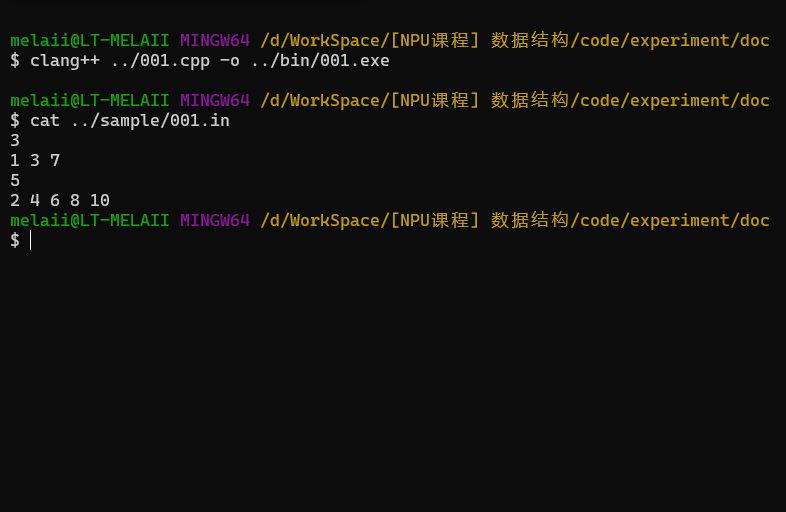
\includegraphics[width=125mm,height=80mm]{./assets/DS01-1}
		\caption{前置环境}
	\end{minipage}
\end{figure}
~\\~\\
\begin{figure}[H]
	\begin{minipage}[t]{\linewidth}
		\centering
		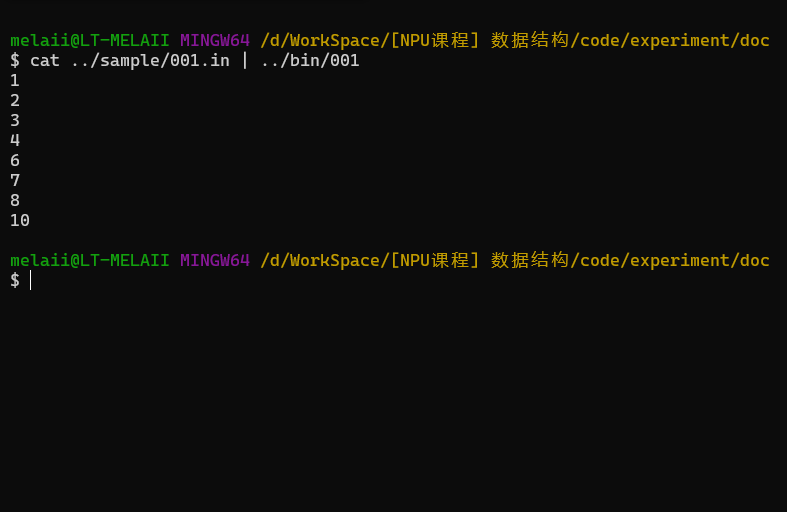
\includegraphics[width=125mm,height=80mm]{./assets/DS01-2}
		\caption{结果输出}
	\end{minipage}
\end{figure}

\subsection*{五、实验总结}
本次实验难度较低,实验目标本身无太大价值,完成实验也不需要耗费太大的精力。除开锻炼对顺序表这一数据结构使用的熟练度,我认为该实验存在附加价值,也即认识到当前算法不仅仅局限于顺序表,并可以在复杂度不变的情况下推广到线性表这一范畴。

~\\
\zihao{-4}
\textbf{教师评语:}
~\\
\textbf{实验成绩:}

\begin{flushright}
\mbox{指导教师签名:\qquad\qquad} \\
\mbox{批阅日期:\qquad\qquad}
\end{flushright}


\end{document}